\def\CC{{C\nolinebreak[4]\hspace{-.05em}\raisebox{.4ex}{\tiny\bf ++}}}

% TODO : NAME
% Copy, s/NAME/yourname/
%======================================================================
% lookup col 1 vs. col 2
\begin{frame}\frametitle{Integrating \textit{Prometheus} into \textit{mirgecom}}
Main components to consider for integration:
\begin{multicols}{2}
\begin{itemize}
  \item Code generator
  \begin{itemize}
    \item \plusplus{C} command-line utility 
    \item XML $\rightarrow$ \textit{Prometheus}(\textit{Cantera}) $\rightarrow$ Python API 
  \end{itemize}
  \item Mixture API
  \item Physics
  \begin{itemize}
    \item Thermodynamics (mixture EOS)
    \item Chemistry (species production rates)
    \item Transport (``advanced'' \& mixture-averaged properties)
  \end{itemize}
\item \textit{Cantera} TPL
\end{itemize}
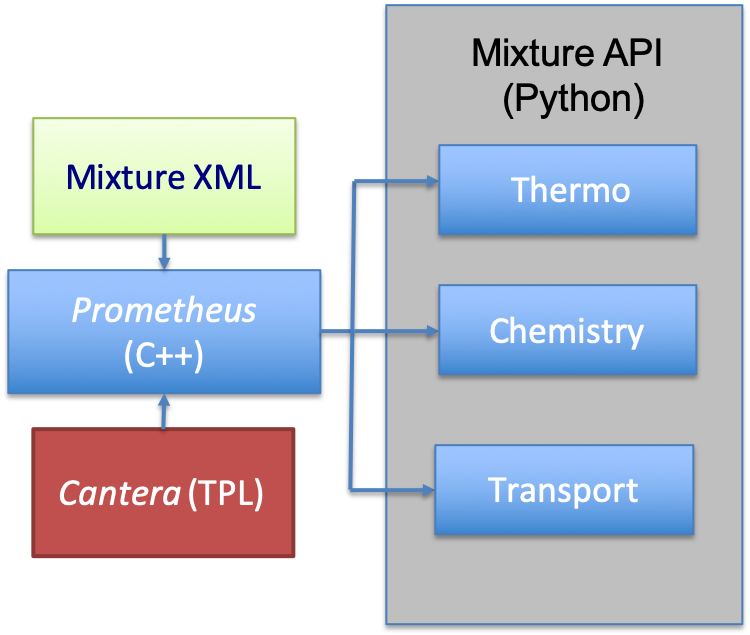
\includegraphics[width=.5\textwidth]{figures/prometheus_cartoon.png}
\end{multicols}
\end{frame}

% official faculty ref. by name?
\begin{frame}\frametitle{A little about \textit{mirgecom}}
\begin{multicols}{2}
\begin{itemize}
  \item \textit{mirgecom}: Python package implements CEESD production simulation API
  \item CEESD community code: \href{https://github.com/illinois-ceesd/mirgecom}{(\textcolor{blue}{https://github.com/illinois-ceesd/mirgecom})}
  \item Builds on several pre-existing packages; most notably A.K.'s suite of Python tools
  \item Users' main interface to engaging CEESD MIRGE machinery to run on modern platforms
\end{itemize}
\end{multicols}
\begin{center}
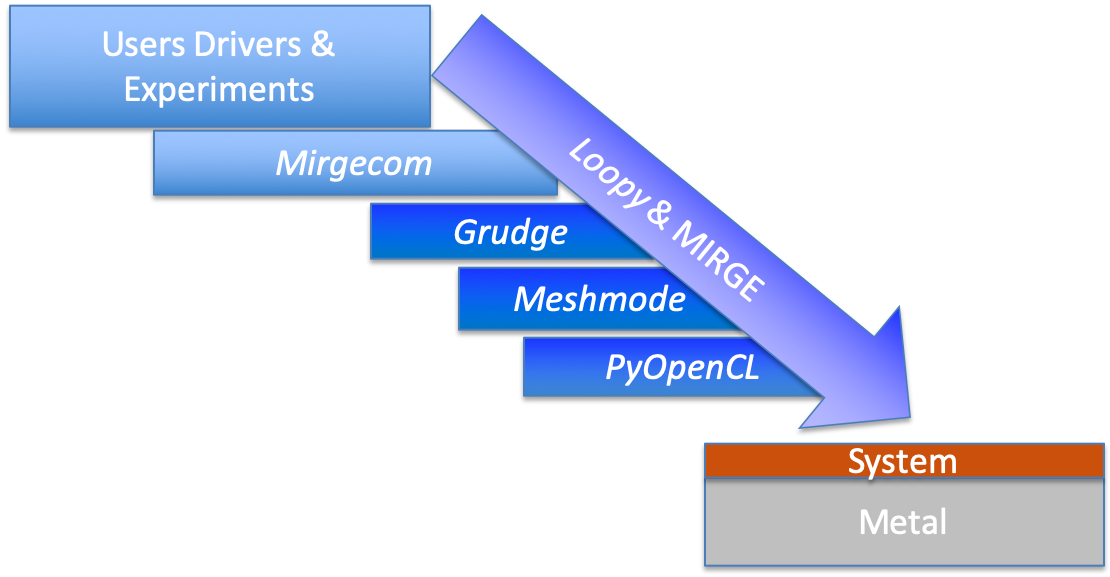
\includegraphics[width=.7\textwidth]{figures/mirgecom_cartoon.png}
\end{center}
\end{frame}

\begin{frame}\frametitle{Plan for \textit{Prometheus} code generation}
\begin{multicols}{2}
\begin{itemize}
  \item Port \textit{Prometheus} to Python
  \item User provides mixture XML input
  \item \textit{Mirgecom} interfaces \textit{Prometheus} Python package to generate mixture API inline
  \item \textit{Prometheus} Python package depends on \textit{Cantera}
\end{itemize}
\end{multicols}
\begin{center}
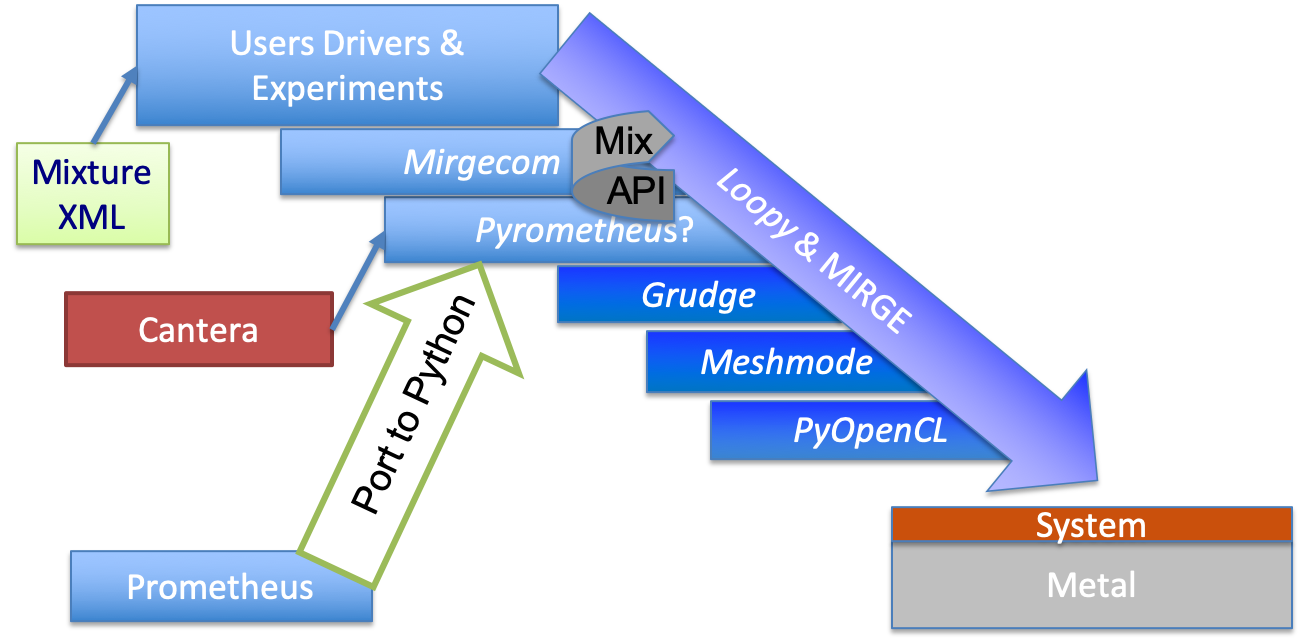
\includegraphics[width=.8\textwidth]{figures/ultimate_integration.png}
\end{center}
\end{frame}

\begin{frame}\frametitle{Planning for the plan - partial integration}
\begin{multicols}{2}
\begin{itemize}
  \item Use \textit{Prometheus} as-is, generate Mixture API to file 
  \item Use Mixture API directly in \textit{mirgecom}
  \item Useful for testing and development of \textit{mirgecom} components that use Mixture API (regardless of source)
  \item Far less convenient to use (from user's perspective)
\end{itemize}
\end{multicols}
\begin{center}
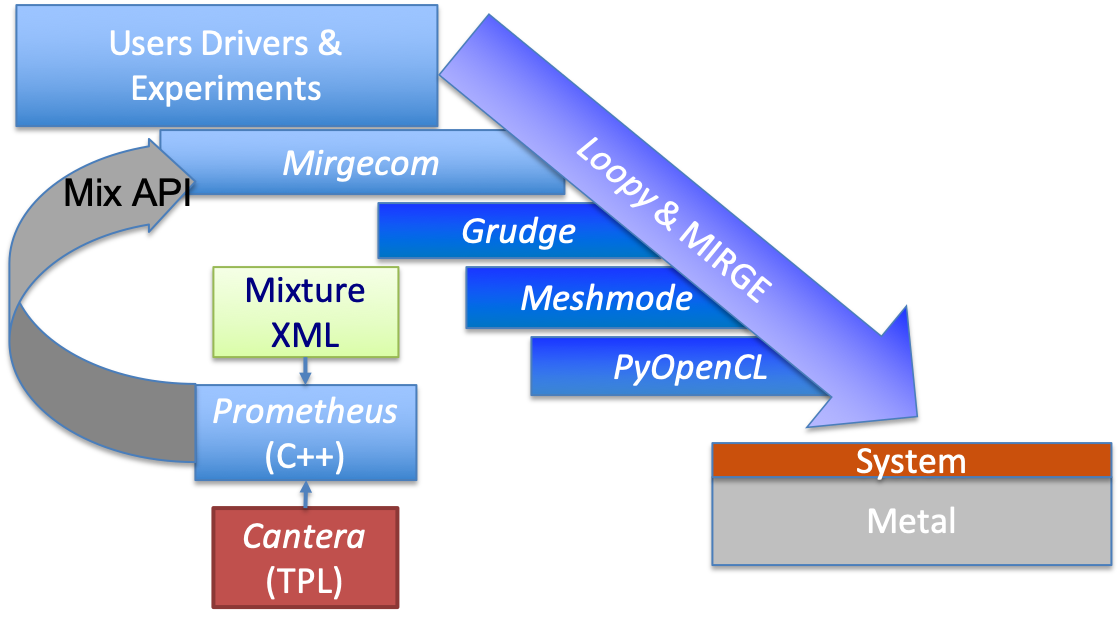
\includegraphics[width=.8\textwidth]{figures/partial_cartoon.png}
\end{center}
\end{frame}

%\begin{frame}\frametitle(Integrating \textit{Prometheus} code generator}
%\begin{multicols}{2}
%\begin{itemize}
%   \item Integration options:
%   \begin{itemize}
%      \item Full integration - \textit{mirgecom} ingests XML, uses \textit{Prometheus} to generate mechanism, %including mechanism in \textit{mirgecom} library
%      \item Partial integration - \textit{Prometheus} pre-generates mechanism for inclusion of interface into %\textit{mirgecom} library
%      \item Non-integration - \textit{Prometheus} stand-alone library implements one or more mechanisms and is% used as a substrate library by \textit{mirgecom} 
%   \end{itemize}
%    \item Staged integration - partial $\rightarrow$ full
%   \item Tests we can do right away (regardless of integration level):
%   \begin{itemize}
%      \item Pre-generated mechanism Python code inclusion (\textit{mirgecom} build and run)
%      \item Pre-generated mechanism function invocations (smoke tests \& screening)
%   \end{itemize}
%\end{itemize}
%\end{multicols}
%\end{frame}

\begin{frame}\frametitle{\textit{Prometheus} Mixture API $\rightarrow$ \textit{mirgecom} EOS}
\begin{multicols}{2}
\begin{itemize}
   \item \textit{Mirgecom} EOS interface (\href{https://mirgecom.readthedocs.io/en/latest/operators.html#equations-of-state}{(\textcolor{blue}{https://mirgecom.readthedocs.io/en/latest/operators.html#equations-of-state})})
   \item \textit{Prometheus} Mixture API thermo properties functions:
   \begin{itemize}
      \item get\_temperature(e, Y, Tguess) $\rightarrow (T, Cp_{mix}, R_{mix})$
      \item get\_pressure(Y, T) $\rightarrow P_{mix}$ 
      \item get\_mix\_cp(T, Y) $\rightarrow (Cp_{mix})$ 
      \item get\_mix\_cv(T, Y) $\rightarrow (Cv_{mix})$
      \item get\_mix\_e(T, Y) $\rightarrow (e)$
      \item get\_mix\_enthalpy(T, Y) $\rightarrow (h_{mix})$
      \item get\_species\_cp\_R(T) $\rightarrow (Cp_{i})$ 
      \item get\_species\_enthalpies(T, Y) $\rightarrow (h_{i})$
   \end{itemize}
%   \item Special considerations
%   \begin{itemize}
%      \item Species ordering, naming
%      \item Buffer species handling
%   \end{itemize}
   \item Potential tests in inviscid setting:
   \begin{itemize}
     \item Species-specific mixture tests (i.e. one species-at-a-time)
     \item Calorically perfect mixture - Compare Prometheus vs. \textit{mirgecom}@CPEOS
     \item Thermally perfect mixture with linear $Cp_i$ - test temperature inversion vs. analytic? 
   \end{itemize}
\end{itemize}
\end{multicols}
\end{frame}

\begin{frame}\frametitle{Wrappers for \textit{Prometheus} EOS}
Create \textit{mirgecom}-EOS-compatible wrappers for \textit{Prometheus} interface functions.
\begin{itemize}
\item get\_pressure(state)
\item get\_temperature(state)
\item get\_internal\_energy(state)
\item get\_speed\_of\_sound(state)
\end{itemize}
\end{frame}

\begin{frame}\frametitle{\textit{Prometheus} chemistry \& transport}
\begin{itemize}
\item Chemistry - get\_net\_production\_rates($\rho$, T, Y) $\rightarrow (\dot{\omega}_i)$
\item For explicit integration - directly feeds species source terms $S_i = (W_i \dot{\omega}_i)$
\item Transport
   \begin{itemize}
      \item Species:  $(\kappa_i, \mu_i, D_{ij})$
      \item Mixture: $(\kappa, \mu, D_i)$
   \end{itemize}
\end{itemize}
%\end{multicols}
\end{frame}

\begin{frame}\frametitle{\textit{Prometheus} / \textit{mirgecom} wishlist}
\begin{itemize}
   \item get\_species\_index(species\_name) - useful for coding the interface/wrappers
   \item get\_species\_names - for I/O, viz/analysis
\end{itemize}           
\end{frame}

\begin{frame}\frametitle{Reactive Flow Equations}
  \begin{align*}
    \pop{\rho}{t} + \Grad\cdot\pp{ \rho \bvec{u} } &= 0 \\
    \pop{ \rho\bvec{u} }{t} + \Grad\cdot\pp{ \rho \bvec{u}\bvec{u} } &= -\Grad p + \Grad\cdot\bvec{\tau} \\
    \pop{ \rho E }{t} + \Grad\cdot\pp{ \rho E \bvec{u} } &= -\Grad\cdot\pp{ p\bvec{u} } + \Grad\cdot\pp{ \bvec{\tau} \cdot \bvec{u} } - \Grad\cdot\bvec{q} \\
    \pop{\rho Y_{i}}{t} + \Grad\cdot\psq{ \rho Y_{i}\pp{ \bvec{u} + \bvec{V}_{i} } } &= W_{i}\dot{\omega}_{i},\quad i = 1,\dots,N
  \end{align*}
  \begin{align*}
    \bvec{\tau} = 2\mu\psq{ \mathbf{S} - \frac{1}{3}\pp{ \Grad\cdot\bvec{u} }\mathbf{I} }\\
    \bvec{q} = -\kappa\Grad T + \sum_{i = 1}^{N}\rho Y_{i} h_{i}\bvec{V}_{i} \\
    Y_{i}\bvec{V}_{i} = \frac{D_{im}W_{i}}{W}\Grad X_{i}\\
  \end{align*}
\end{frame}
%======================================================================

%======================================================================
\begin{frame}\frametitle{Chemical Source Term}
  \begin{align*}
    \omega_{i} &= \nu_{ij}R_{j} \\
    R_{j} &= k_{j}(T)\psq{ \prod_{m = 1}^{N}\pp{\frac{\rho Y_{m}}{W_{m}}}^{\nu_{mj}^{\prime}} - \frac{1}{K_{j}(T)}\prod_{n = 1}^{N}\pp{\frac{\rho Y_{m}}{W_{m}}}^{\nu_{nj}^{\prime\prime}}  } \\
    K_{j}(T) &= \pp{ \frac{p_{0}}{RT} }^{\sum_{i = 1}^{N}\nu_{ij}}\exp\psq{ -\sum_{m = 1}^{N} \frac{\nu_{mj}g_{m}(T)}{RT} } \\
    k_{j}(T) &= A_{j} T^{b_{j}}\exp\pp{ -\frac{E_{a,j}}{RT} } \\
    \frac{g_{i}(T)}{RT} &= \frac{h_{i}(T)}{RT} - \frac{s_{i}}{R} \\
    \frac{h_{i}(T)}{RT},\,\frac{s_{i}(T)}{R} &: \text{NASA polynomials}
  \end{align*}
\end{frame}
%======================================================================
\end{document}
